\documentclass[11pt]{scrartcl}

\usepackage{ucs}
\usepackage[utf8x]{inputenc}
\usepackage[T1]{fontenc}
\usepackage[ngerman]{babel}
\usepackage{amsmath,amssymb,amstext}
\usepackage{graphicx}
\usepackage[justification=RaggedRight, singlelinecheck=false]{caption}
\usepackage{tikz}
\usepackage[square,sort,comma,numbers]{natbib}
\usepackage{url}

\title{Fortgeschrittenen Praktikum Teil 2: PI}
\subtitle{Versuch 4: Magnetische Resonanz \\ Betreuer: Paul Eibisch}

\author{Gruppe 1: Reinhold Kaiser, Florian Stoll}

\date{09.07.2018}

\begin{document}
\maketitle
\newpage
\tableofcontents
\newpage
\bibliographystyle{alphadin}
\section{Target}

\section{Theoretische Grundlagen}
Die grundlegende Eigenschaft für den vorliegenden Versuch ist der Spin. Als rein quantenmechanische Eigenschaft besitzt der Spin kein klassisches Analogon und kann zwar mit dem Eigendrehimpuls eines Körpers verglichen aber nicht gleichgesetzt werden. Wichtige Unterschiede liegen vor allem in der Quantelung des Spins und in der fehlenden räumlichen Ausdehnung der quantenmechanischen Teilchen wie z.B. dem Elektron. Der Spin eines Teilchens lässt sich über zwei Kenngrößen beschreiben, wobei man üblicherweise die z-Komponente und den Betrag des Spin-Vektors auswählt. Im Fall eines Spins I lauten diese:

\begin{align}
\vert I \vert = \sqrt{I\left(I+1)\right)\hbar^2} \\
I_z=m_I \hbar \\
m_I \in [-I,I]
\end{align}

Über die magnetische Quantenzahl $m_I$ ergeben sich dann $2I+1$ verschiedene Einstellmöglichkeiten, die jedoch in Abwesenheit externer Felder alle energetisch entartet sind.

Wie jeder Drehimpuls geladener Teilchen ist natürlich auch der Spin mit einem magnetischen Moment verbunden, über das er z.B. mit einem externen Magnetfeld wechselwirken kann. Den teilchenabhängigen Proportionalitätsfaktor zwischen Spin und magnetischem Moment bezeichnet man als gyromagnetisches Verhältnis $\gamma$. Dieses ist schon in klassischer Rechnung bekannt und ergibt sich im Fall eines Elektrons mit Ladung $-e$, Masse $m_e$ und klassischem Bahndrehimpulses L zu:

\begin{align}
\overrightarrow{\mu_L}=\gamma \cdot \overrightarrow{L} = \frac{q}{2m}\cdot \overrightarrow{L}=\frac{-e}{2m_e}\cdot \overrightarrow{L} = -\mu_B \cdot \frac{\overrightarrow{L}}{\hbar}
\end{align}

Dabei bezeichnet $\mu_B=\frac{e\hbar}{2m_e}$ das sogenannte Bohrsche Magneton, eine Naturkonstante. 

Das gyromagnetische Verhältnis im Fall des Spins lässt sich prinzipiell nach obigem Beispiel berechnen. Aus Messungen und auch aus relativistischen Quantenmechanik-Rechnungen lässt sich jedoch feststellen, dass obige Gleichung im Fall des Spins noch um den Landé-Faktor g ergänzt werden muss. Dieser ist ebenfalls teilchenabhängig und gibt eine unterschiedlich starkes magnetisches Moment im Bezug auf den Spin an. Im Fall eines Elektrons und eines Atomkerns lautet die Beziehung zwischen den Spins S (Elektronspin) bzw. I (Kernspin) und dem jeweiligen magnetischen Moment wie folgt:

\begin{align}
\overrightarrow{\mu_S}=-\frac{\mu_B}{\hbar}\cdot \overrightarrow{S}\cdot g \\
\overrightarrow{\mu_I}=\frac{e\hbar}{2m_p}\cdot \frac{\overrightarrow{S}}{\hbar}\cdot g 
\end{align}

Die Größe $\frac{e\hbar}{2m_p}$ bezeichnet man analog zum Bohrschen Magneton als Kernmagneton $\mu_N$. Um auch bei verschiedenen Teilchen weiter mit diesen beiden Naturkonstanten rechnen zu können, definiert man alle Abweichungen von dieser Größe in den jeweiligen g-Faktor des untersuchten Teilchens. Im Fall des Protons beträgt dieser ungefähr: $g \approx 5,586$.

Durch Vergleich der Formeln lässt sich nun das gyromagnetische Verhältnis in Beziehung zum Landé-Faktor g setzen:

\begin{align}
\gamma = \frac{\mu_N g}{\hbar}
\end{align}

Legt man nun ein konstantes externes Magnetfeld in z-Richtung an, koppelt das magnetische Moment eines Kerns an das Magnetfeld und die Entartung der Zustände mit verschiedener Quantenzahl $m_I$ wird aufgehoben. Diesen Effekt bezeichnet man als Zeeman-Effekt, dessen Energien $E_Z$ sich wie folgt berechnet:

\begin{align}
E_Z = -\overrightarrow{\mu}\cdot\overrightarrow{B}=-\mu_N \cdot g \cdot B_0 \cdot m_I \\
\overrightarrow{B}=B_0\cdot \overrightarrow{e_z}
\end{align}

Wie zu erkennen nimmt die Energiedifferenz zwischen den Zuständen linear mit dem angelegten Magnetfeld zu, sodass sich im Fall eines Kernspins $I=\frac{1}{2}$ der in Abbildung \ref{prop} dargestellte Verlauf ergibt:

\begin{figure}[htbp] 
     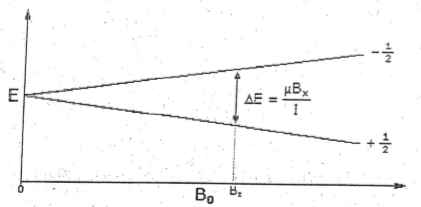
\includegraphics{Aufspaltung.png}
  \caption{Proportionalität der Energiedifferenz zwischen zwei Zeemann-Zuständen \cite{anleitung}}
  \label{prop}
\end{figure}

Die Energiedifferenz zwischen den beiden Zuständen ergibt sich weiterhin zu:
\begin{align}
\Delta E = \vert E_{m=\frac{1}{2}} - E_{m=-\frac{1}{2}} \vert = \mu_N \cdot g \cdot B_0 = \hbar \cdot \gamma \cdot B_0 = \hbar \omega_L
\end{align}
$\omega_L$ bezeichnet dabei die der Energiedifferenz entsprechenden Frequenz, mit der sich Übergänge zwischen den beiden Zuständen anregen lassen. Mit dem Zahlenwert für das Kernmagneton $\mu_N=5,05 \cdot 10^{-27} \frac{J}{T}$ wird ersichtlich, dass die so entstehenden Energiedifferenzen sehr klein (ungefähr im $\mu eV$-Bereich) liegen.

Liegen die Vektoren $\overrightarrow{I}$ und $\overrightarrow{B}$ nun nicht parallel zueinander, stellt sich ein Effekt ein, den man ebenfalls schon klassisch betrachten kann. Der Drehimpuls-Vektor präzessiert dabei wie in Abbildung \ref{Larmor} dargestellt  um den Magnetfeld-Vektor mit der sog. Larmor-Frequenz $\omega$. Diese bestimmt sich über vektorielle Rechnungen zu:
\begin{align}
\omega_L=B_0 \cdot \gamma
\end{align}
Die Bezeichnung $\omega_L$ ist in obiger Formel für die Energiedifferenz ist dabei nicht zufällig gewählt, da dies ebenfalls genau die Larmor-Frequenz ist. 

\begin{figure}[htbp] 
     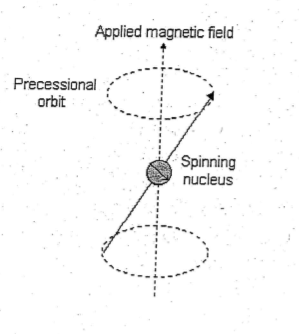
\includegraphics{Larmor.png}
  \caption{Larmor-Präzession eines Drehimpulsvektors um ein angelegtes Magnetfeld \cite{anleitung}}
  \label{Larmor}
\end{figure}

Für das zu untersuchende Phänomen der Kernspinresonanz müssen wir noch die Besetzungen der beiden Zuständen im Fall $I=\frac{1}{2}$ betrachten. Diese lassen sich durch die Boltzmann-Verteilung beschreiben:
\begin{align}
\frac{N_{m_{I+1}}}{N_{m_I}} \sim e^{-\frac{\Delta E}{k_BT}}
\end{align}

Wenn wir nun unsere größenordnungsmäßig kleine Energieaufspaltung zwischen den beiden Zuständen berücksichtigen nähert sich die Boltzmann-Verteilung nahezu zu 1. Wäre dies exakt der Fall, würden wir keinerlei Resonanz-Effekte messen, da sich die beiden Effekte der Photon-Absorption und der stimulierten Emission gerade aufheben würden. Dies ist aber nicht exakt der Fall, denn natürlicherweise liegen mehr Kernteilchen im energetisch niedrigeren Zustand vor. Durch Anregung mit der Resonanzfrequenz $\omega_L$ lassen sich diese Kernteilchen auf den energetisch höheren $m_I=-\frac{1}{2}$-Zustand anheben und wir können eine Absorption der Strahlung im entsprechenden Frequenzbereich beobachten. Bestrahlt man eine Probe längere Zeit mit der entsprechenden Frequenz, so stellt sich nach und nach das oben erwähnte Gleichgewicht ein und anschließend wird keine Absorption mehr  beobachtet. Mit der Zeit stellt sich nach Abstellen der Strahlung wieder der Grundzustand ein, da die Kernteilchen über Spin-Spin- oder Spin-Gitter-Wechselwirkungen wieder Energie abgeben können. Charakteristisch für diese Effekte sind die sogenannten Relaxationszeiten, welche zwischen $10^{-4}s$ und mehreren $10^4s$ liegen können.

\section{construction of experiment and used devices}


\section{Execution and results}

\section{Anwendungen der NMR}
Die NMR fidnet in vielen unterschiedlichen Bereichen Anwendung, wesegen hier 3 verschiedene Anwendungen der NMR vorgestellt und erläutert werden sollen.

\subsection{NMR in der Medizin (MRT)}
Die Magnetresonanztomografie (MRT) ist ein bildgebendes Verfahren zur Darstellung von Organen oder Gewebe des Körpers. Ausgenutzt wird dabei der Kernspin der Protonen, sodass die Protonendichte oder unterschiedliche Relaxationszeiten die unterschiedlichen Gewebearten bzw. Kontraste darstellen.
\subsubsection*{Aufbau einer typischen Anlage zur MRT}
\begin{figure}[htbp] 
     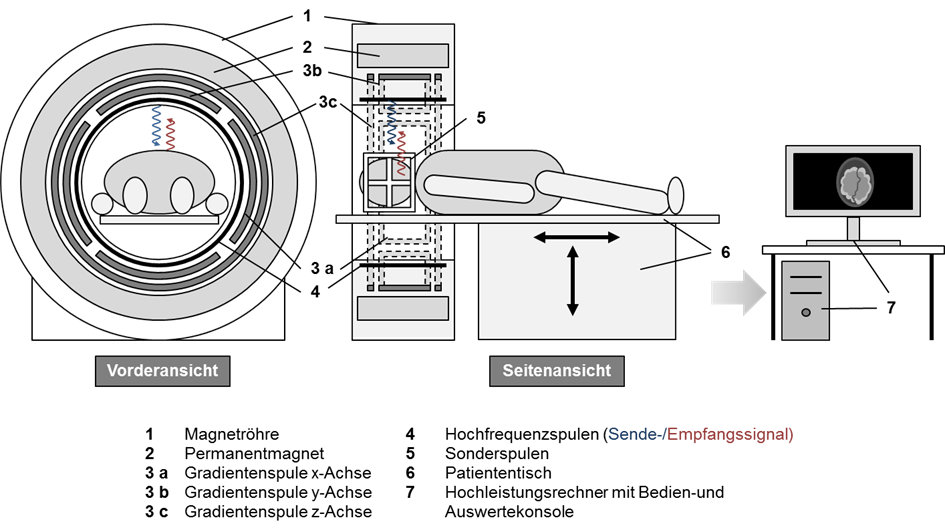
\includegraphics[width=0.99\textwidth]{mrt_aufbau.png}
  \caption{Schematischer Aufbau einer MRT-Anlage \cite{mrt}}
  \label{mrt_aufbau}
\end{figure}
In Abblidung \ref{mrt_aufbau} sieht man den Aufbau einer typischen MRT-Anlage. Die entscheidenden Elemente sind Gradientenspulen und die Hochfrequenzspulen, sowie der Permanentmagnet, der die Aufpaltung der Kernspinlevel der Protonen verursacht.
\subsubsection*{Funktionsprinzip der MRT}
Der Permanentmagnet ist ein supraleitender mit Helium gekühlter Magnet, der ein nahezu räumlich konstantes Magnetfeld von $1,5T$ oder $3T$ liefert. Durch die Hochfrequenzspule wird die Magnetisierung des Patienten kurzzeitig verändert, der Übergang in die ursprüngliche Magnetisierung erfolgt dann durch Aussenden Strahung, welche von der Hochfrequenzspule empfangen wird. Die räumliche Zuordnung erfolgt durch die Gradientenspulen, die in x-, y-, und z-Richtung ausgerichtet sind. DIe Sonderspulen verbessern das Signal und am Hochleistungsrechner wird dann aus den Daten das Bild erstellt. 

\subsection{NMR in der Chemie (Strukturanalyse)}
In der Chemie wird die NMR genutzt, um die Struktur von Molekülen genauer zu untersuchen. Entscheidend ist, dass die Resonanzen in unterschiedlichen Bindungen in ihrer Frequenz unterschiedlich verschoben werden.
\subsubsection*{Chemische Verschiebung}
Die Elektronen, die den Atomkern umgeben, bewegen sich entsprechend dem angelegten Magnetfeld $B_0$, da sie geladene Teilchen sind. So generieren sie ein viel kleineres entgegengerichtetes Magnetfeld, was den Kern vom Magnetfeld teilweise abschirmt. $B_0$ muss also leicht erhöht werden, damit Resonanz bei einer gegebenen Radiofrequenz auftritt. Unterschiedliche Bindungen führen zu unterschiedlichen Abschirmungen, sodass die Verschiebung des Magnetfelds spezifisch zu ein Referenz in $ppm$ angegeben werden kann. In Protonen-NMR wird als Referenz Tetramethylsilan (TMS) verwendet, da einen scharfen Peak im Spektrum hat und weitere positive chemische Eigenschaften besitzt.
\subsubsection*{Kopplungsstruktur der NMR-Spektren}
In der Wasserstoff-NMR-Spektroskopie tritt ein Effekt auf, der durch das Koppeln der benachbarten Protonen entsteht. Das benachbarte Proton kann einen zum angelegten Magnetfeld parallelen oder antiparallelen Kernspin haben. Dadurch teilt sich der Zustand des anderen Protons zu einem Dublett auf. Ganz allgemein ergeben sich für $n$ Nachbarn $ n + 1$ neue Zustände, die im NMR-Spektrum zu sehen sind.

\subsection{NMR in der Festkörperphysik}
\subsubsection*{Besonderheiten der Festkörper-NMR}
Für Materialien, in denen die Atome oder Moleküle keine oder nur eine sehr geringe Beweglichkeit haben, können die richtungsabhängigen Interaktionen der einzelnen Atomkerne mit Hilfe der NMR-Spektroskopie aufgelöst werden. Anders gesagt verändern die richtungsabhängigen Interaktionen die Kernspin-Energielevels.
\subsubsection*{Magic-Angle-Spinning-NMR}
Durch die eben beschriebenen anistropen Wechselwirkungen treten Linienverbreiterungen auf, die es erschweren, das NMR-Spektrum zu analysieren. Eine Methode, um die Signalqualität zu verbessern ist das Magic-Angle-Spinning (MAS). Dabei wird die Probe um eine Rotationsachse rotiert, die in einem Winkel von ca. $54,74°$ zu dem externen Magnetfeld ausgerichtet ist. Die anisotropen Wechselwirkungen können so herausgemittelt werden und die Linienbreiten des Spektrums wird deutlich schärfer.
\subsubsection*{Knight-Shift}
Der Knight-Shift ist ein Effekt, der auftritt, wenn man die Resonanzfrequenz von einem Atom in einem Nichtmetall und in einem Metall vergleicht. Ähnlich wie bei der chemischen Verschiebung wird dem äußeren Magnetfeld ein effektives Magnetfeld überlagert, was durch die Ausrichtung der Spins der Leitungselektronen entsteht, wenn ein externes Magnetfeld angelegt ist. So wird die Resonanzfrequenz um einen Betrag der Größenordnung ein Promille verschoben.


\section{Zusammenfassung/Fazit}


\bibliography{Literaturverzeichnis}



\end{document}
